\documentclass[cameraready]{ieeeconf}

\usepackage{booktabs}

\usepackage{graphicx}

\usepackage{amsmath}

\title{Sketch2Face Cross Modal Face Retrieval on the CUFS CUHK Subset}

\addauthor{Ipsita}{1}

\addaffiliation{1}{B.Tech in Artificial Intelligence and Machine Learning, Lovely Professional University, Punjab, India}

\begin{document}

\maketitle

\begin{abstract}

Matching a hand-drawn face sketch to a photographic gallery is difficult because identity must be preserved across different image domains. This project implements a cross-modal retrieval system using modality-specific residual input adapters, a shared ImageNet-pretrained ResNet-18, and a normalized 256-dimensional projection trained with a symmetric contrastive objective. A public CUFS mirror was audited and found to contain 188 usable CUHK sketch-photo pairs rather than the 606 pairs advertised in its description. We therefore evaluate only the CUFS CUHK subset, using 114 training, 37 validation, and 37 test identities. Against all 37 held-out photos, the primary model achieves 72.97\% rank-1, 89.19\% rank-5, and 100.00\% rank-10 accuracy, compared with 27.03\% rank-1 for a frozen pretrained baseline. Across three training seeds, rank-1 is 69.37\% with a sample standard deviation of 3.12 percentage points. These findings support the value of paired fine-tuning under this small closed-set protocol, but do not establish performance on full CUFS, large galleries, eyewitness sketches, or composite forensic sketches.

\end{abstract}

\section{Introduction}

A sketch-based face retrieval system receives a drawing and searches a gallery of photographs for the same person. The output is an ordered candidate list rather than a generated face image or a class from a fixed set of training identities. The central challenge is domain shift: pencil strokes emphasize contours, whereas photographs contain illumination, texture, and color. Features that separate people within photographs may not remain stable in drawings. A useful embedding must retain identity-related structure while reducing sensitivity to modality.


The project objective is to implement, test, and document a reproducible cross-modal matcher with rank-k evaluation. Its contributions are engineering and experimental: explicit data-pair auditing, identity-disjoint partitions, a lightweight shared-encoder model, a controlled frozen-feature baseline, repeated training seeds, an adapter ablation, and an application that uses the same inference path as evaluation. The architecture combines established methods; no novel algorithm or state-of-the-art performance is claimed.


Although motivated by forensic sketch search, the evaluated material consists of viewed artist sketches. Such drawings are made while observing the corresponding photograph, unlike sketches reconstructed from witness memory or assembled from facial components. Consequently, the application is a college research prototype and its measured scope must remain explicit.


\section{Related work}

Wang and Tang \cite{ref1} investigated face photo-sketch synthesis and recognition, providing a foundation for work on matching the two modalities. Zhang, Wang, and Tang \cite{ref2} studied coupled information-theoretic encoding for photo-sketch recognition. These studies motivate learning a representation shared by drawings and photographs rather than relying solely on raw appearance. Their published recognition numbers are not used as direct numerical baselines here because training protocols, preprocessing, and gallery composition can differ.


ResNet \cite{ref3} provides residual visual representations that can be adapted from large-scale image pretraining to a smaller target dataset. Symmetric contrastive alignment, as used for paired modalities in CLIP \cite{ref4}, supplies the form of the bidirectional objective employed here; this project does not use CLIP weights, text inputs, or a language encoder. AdamW \cite{ref5} provides decoupled weight decay for optimization. The present implementation tests whether adapting pretrained image features to genuine sketch-photo pairs improves retrieval under a fixed local protocol.


\section{Dataset audit and experimental split}

Full CUFS is described as 606 identities: 188 CUHK students, 123 AR identities, and 295 XM2VTS identities [1, 2, 6]. The official archive page returned HTTP 500 during acquisition. We downloaded public Kaggle mirror version 1 \cite{ref6} and audited its actual contents instead of accepting the listing total. It contained 188 cropped photographs and 188 matching CUHK sketches, original-resolution copies, and 1,194 additional sketches without corresponding photo pairs. AR and XM2VTS pairs were unavailable in this copy. Only the verified CUHK pairs were included; this experiment is not a full-CUFS benchmark.


Pairing uses normalized filenames, not directory order. Names are made case-insensitive; the sketch suffix -sz1 is removed; F2-/M2- groups map to the corresponding f-/m- photo groups, while f1-/m1- remain unchanged. The resulting 188 one-to-one mappings were checked for readable images, minimum dimensions, exact decoded-pixel duplicates, and identity collisions. Representative pairs were inspected visually. A provenance record preserves the download URL, archive checksum, version, exclusions, and original-author rights notice.


A fixed seed of 42 partitions identities into 114 training, 37 validation, and 37 test subjects. Both images of each subject stay in one split. This is a custom 60/20/20 split with integer rounding, not an official published CUFS protocol. The manifest records every identity, source, split, image path, and SHA-256. Input files are rechecked before training or evaluation, and checkpoints must match the manifest fingerprint. This prevents accidental reuse of training identities or changed files in the reported test.


\section{Proposed system}

Images are corrected for EXIF orientation, converted to RGB, then to three-channel grayscale, resized from the supplied 200 by 250 face crops to 224 by 224, and normalized using the ImageNet mean and standard deviation. The same deterministic preprocessing is used for validation, testing, and application inference. Training adds paired horizontal flips and independent small affine perturbations: rotation up to five degrees and translation up to 2.5 percent. No landmark detector or automatic alignment is implemented; uploaded inputs should already be comparably cropped.


For modality m, the input is transformed as x + A\_m(x), where A\_m is a zero-initialized 1 by 1 convolution with three input and output channels and no bias. The two adapters contain 18 parameters in total and initially act as identity mappings. A shared ResNet-18 \cite{ref3} produces a 512-dimensional pooled feature. The projection head applies Linear(512,256), ReLU, and Linear(256,256). L2 normalization places the final embeddings on the unit hypersphere. These small adapters adjust channel combinations; they do not reconstruct a photo or align facial landmarks.


Let S and P be matrices of normalized sketch and photo embeddings for B distinct paired identities. Similarity logits are L = S P\textasciicircum{}T / tau, with tau = 0.07. The target label for row i is i. The loss is one half of CE(L, labels) plus CE(L\textasciicircum{}T, labels), following a symmetric paired contrastive formulation \cite{ref4}. Matched pairs are positives and other identities in the batch are negatives. At inference, cosine similarity z\_sketch dot z\_photo ranks candidates; no claim of calibrated identity probability is made.


\begin{equation}

\mathcal{L}=\tfrac{1}{2}\left[\mathrm{CE}(Z_s Z_p^\top/\tau,y)+\mathrm{CE}(Z_p Z_s^\top/\tau,y)\right],

\end{equation}

where $y_i=i$, $\tau=0.07$, and rows of $Z_s$ and $Z_p$ are normalized embeddings.

\section{Experimental setup}

All trained models run for 20 epochs with batch size 32, AdamW \cite{ref5}, weight decay 0.0001, and gradient norm clipping at 5. Adapters and projection use learning rate 0.0003; the encoder uses 0.00003. Epochs 1 through 3 freeze the full encoder. Epochs 4 through 20 unfreeze only its final residual stage. Batch-normalization running statistics remain frozen to reduce instability on the small dataset. The best checkpoint maximizes validation rank-1; ties are broken by validation mean reciprocal rank, then the earlier epoch. Test results are never used for selection.


The frozen baseline uses ImageNet-1K V1 ResNet-18 weights, identical preprocessing, and raw L2-normalized 512-dimensional features without adapters or projection. The main matcher is trained with seeds 42, 43, and 44 on the same identity split. Seed 42 is designated as primary before test evaluation. The adapter ablation uses seed 42 and retains the same projection, optimization, and schedule while bypassing both input adapters. The experiment matrix is saved before repeated training and evaluation. Experiments ran locally using Apple MPS; software versions and checkpoint hashes are retained in machine-readable outputs.


Each of the 37 test sketches is compared against all 37 test photographs. Rank-k is the fraction of queries whose correct match appears in the first k candidates; CMC computes this fraction at each rank. Every tied distractor counts ahead of the correct photo, preventing optimistic tie handling. Query-level 95 percent percentile bootstrap intervals use 2,000 resamples. The primary-minus-baseline rank-1 difference uses 10,000 paired query resamples. Training-seed mean and sample standard deviation are reported separately from these fixed-checkpoint intervals.


\section{Results and discussion}

Table I reports every predeclared run. The primary model correctly ranks 27 of 37 photos first (72.97\%), compared with 10 of 37 (27.03\%) for the baseline. Its rank-5 and rank-10 accuracies are 89.19\% and 100.00\%, corresponding to 33 and 37 successful queries. The rank-1 bootstrap interval is [59.46\%, 86.49\%]. The absolute rank-1 gain is 45.95 percentage points, with paired bootstrap interval [27.03, 64.86] percentage points. The matcher recovers 19 queries missed at rank 1 by the baseline, while losing 2 that the baseline ranked correctly. This supports a benefit from paired training in this fixed experiment.


The three matcher runs achieve rank-1 values of 72.97\%, 67.57\%, 67.57\%. The mean is 69.37\% and sample standard deviation is 3.12 percentage points. The repeated seeds share the same training and test identities; they quantify optimization variation rather than generalization across independent splits. The primary model was selected at epoch 20, the final allowed epoch. This does not demonstrate convergence or imply that 20 epochs are optimal.


The no-adapter model reaches 67.57 percent rank-1 and 97.30 percent rank-5. Thus, the primary adapter run improves rank-1 by 5.41 percentage points but has lower rank-5 than the ablation. One ablation seed cannot establish a reliable benefit from adapters, and the observed pattern does not support describing them as uniformly better. The defensible finding is that fine-tuning and projection improve on frozen generic features; the adapters require further controlled investigation.


Ten primary queries fail at rank 1, although every correct match appears by rank 10. The hardest correct match is at rank 10. The CMC comparison and training curves accompany the report. Falling contrastive loss and increasing validation retrieval are consistent with learning, but do not eliminate overfitting concerns. Rank-10 reaches a bootstrap interval of [100,100] percent because every observed query succeeds; this boundary result is not evidence of perfect performance on future identities.


\begin{table}[t]

\centering

\caption{Retrieval accuracy (\%) on 37 test queries and the same 37-photo gallery. Epoch selection uses validation only.}

\label{tab:results}

\small

\begin{tabular}{lrrrr}

\toprule

Model & Epoch & R@1 & R@5 & R@10 \\

\midrule

Frozen baseline & 0 & 27.03 & 51.35 & 72.97 \\

Matcher seed 42 & 20 & 72.97 & 89.19 & 100.00 \\

Matcher seed 43 & 20 & 67.57 & 89.19 & 100.00 \\

Matcher seed 44 & 16 & 67.57 & 91.89 & 100.00 \\

Without adapters & 18 & 67.57 & 97.30 & 100.00 \\

\bottomrule

\end{tabular}

\end{table}

\begin{figure}[t]

\centering

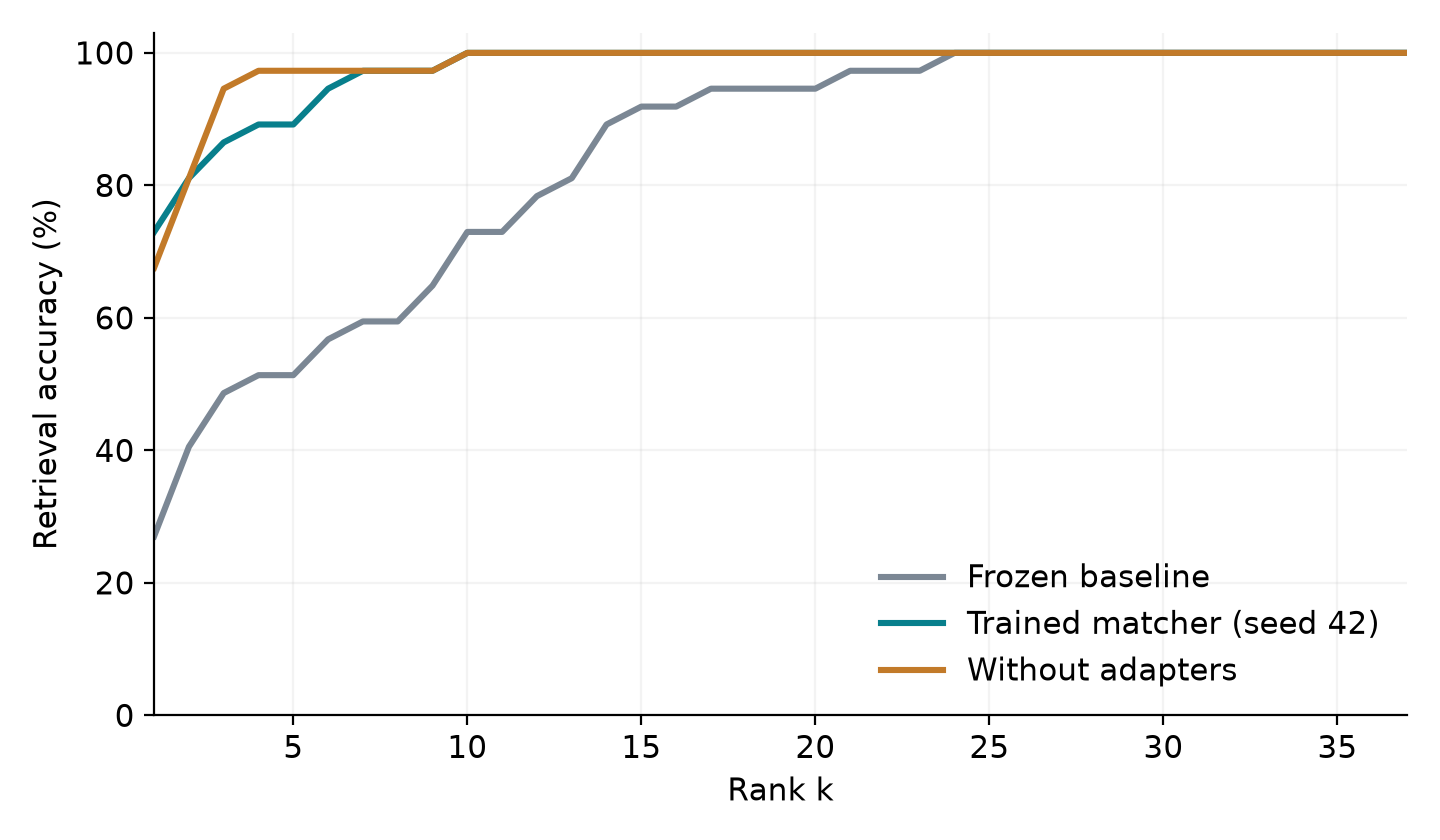
\includegraphics[width=\linewidth]{figures/cmc_comparison.png}

\caption{Measured CMC under the fixed 37-photo test protocol. This figure contains no dataset face images.}

\label{fig:cmc}

\end{figure}

\section{Limitations and responsible interpretation}

The strongest limitation is dataset coverage. Only the CUHK subset is paired and evaluated; AR and XM2VTS, unseen-source transfer, and the complete 606-identity benchmark remain untested. The test contains just 37 identities, so one query changes accuracy by approximately 2.70 percentage points. The gallery is fixed and closed set, making the task easier than searching a large operational database that may not contain the person.


Bootstrap intervals condition on the available gallery and checkpoint. They do not account for demographic coverage, independent sampling of galleries, differences between sketch artists, or witness-memory distortion. ImageNet pretraining is declared, but potential identity overlap has not been independently audited. The dataset does not support a meaningful demographic fairness claim. Retrieval scores must not be used as identity verification, evidence of guilt, or an automatic decision about a person.


Further work should obtain the complete CUFS sources through their owners, predefine larger-gallery and leave-one-source-out protocols, repeat ablations across seeds and splits, and evaluate on an appropriate forensic sketch dataset. Unknown-person rejection would require a separate open-set evaluation and validation-selected thresholds. Gallery-feature caching and automatic face alignment are engineering extensions, not completed experiments.


\section{Conclusion}

Sketch2Face provides a working cross-modal matcher, reproducible experiment pipeline, retrieval application, and rank-k report based on actual data. On a 37-photo held-out gallery drawn from 188 CUHK identities, the primary model achieves 72.97\% rank-1 compared with 27.03\% for frozen pretrained features. The three-seed rank-1 mean is 69.37\%. These results support paired representation learning under this restricted protocol. They do not validate the entire CUFS benchmark or real forensic deployment. The archive audit and recorded experimental limits are part of the findings, not details to omit from the final submission.


\begin{thebibliography}{6}

\bibitem{ref1} X. Wang and X. Tang, "Face Photo-Sketch Synthesis and Recognition," IEEE Transactions on Pattern Analysis and Machine Intelligence, vol. 31, no. 11, pp. 1955-1967, 2009. doi:10.1109/TPAMI.2008.222.

\bibitem{ref2} W. Zhang, X. Wang, and X. Tang, "Coupled Information-Theoretic Encoding for Face Photo-Sketch Recognition," IEEE CVPR, pp. 513-520, 2011.

\bibitem{ref3} K. He, X. Zhang, S. Ren, and J. Sun, "Deep Residual Learning for Image Recognition," IEEE CVPR, pp. 770-778, 2016. \url{https://arxiv.org/abs/1512.03385}.

\bibitem{ref4} A. Radford et al., "Learning Transferable Visual Models From Natural Language Supervision," ICML, PMLR 139, pp. 8748-8763, 2021. \url{https://arxiv.org/abs/2103.00020}.

\bibitem{ref5} I. Loshchilov and F. Hutter, "Decoupled Weight Decay Regularization," ICLR, 2019. \url{https://arxiv.org/abs/1711.05101}.

\bibitem{ref6} Arbaz Khan, "CUHK Face Sketch Database (CUFS)," Kaggle public mirror, version 1, updated October 8, 2020; accessed November 9, 2026. \url{https://www.kaggle.com/datasets/arbazkhan971/cuhk-face-sketch-database-cufs}. Data rights retained by original authors.

\end{thebibliography}

\end{document}
